%\documentclass{ctexart} 使用 ctex 字体
\documentclass[nofonts]{ctexart} % 不用 ctex 字体

\usepackage{xltxtra} % 让 xelatex 支持UTF
\usepackage{graphicx} % 图形库
\usepackage{amsmath} % AMS 的数学符号

% 自定义字体
% 如果使用 ctex 字体,注释掉以下部分.
\setCJKmainfont[
BoldFont={WenQuanYi Zen Hei:style=Regular},
ItalicFont={AR PL KaitiM GB:style=Regular}]
{AR PL UMing CN:style=Light}
\setCJKsansfont{WenQuanYi Zen Hei Sharp:style=Regular}
\setCJKmonofont{WenQuanYi Zen Hei Mono:style=Regular}

\title{Assignment 4:Interpolation}
\author{Xu Yang\\ Computer Science 3220102703}
\begin{document}
\maketitle
\section{Visualization}
\begin{figure}[htbp]
      \centering
      \includegraphics[scale=0.5]{./interp.eps}
      \caption{interpolation graph}
  \end{figure}
\section{Description}
这个程序使用3次样条曲线对这10个点的数据$(x_i,y_i)$进行插值,其中$x_i=i+sin(i)/2,y_i=i+cos(i^2)*3.220102703$
\end{document}
